\section{Исследовательская часть}

\subsection{Технические характеристики}

Технические характеристики устройства, на котором выполнялся замерный эксперимент:
\begin{itemize}[label*=---]
	\item операционная система Windows 11;
	\item память 16 ГБ;
	\item процессор 3,6 ГГц 6-ядерный процессор AMD Ryzen 5000 series 5.
\end{itemize}

Замеры проводились на ноутбуке, включенном в сеть электропитания. 
Во время тестирования ноутбук был нагружен только интегрированной средой разработки и непосредственно выполняемой программой.

\subsection{Пример работы программы}

На рисунке \ref{fig:example} представлен пример работы программы. 

\begin{figure}
	\centering
	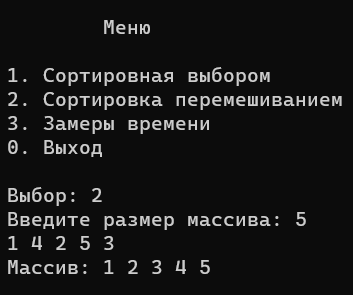
\includegraphics[width=0.4\linewidth]{images/example}
	\caption{Пример работы программы}
	\label{fig:example}
\end{figure}

\newpage

\subsection{Время выполнения реализованных алгоритмов}
Замеры времени работы реализованных алгоритмов для определенного размера массива проводились 1000 раз, при этом каждый раз значения массива генерировались случайно.

Для измерения тактового времени была использована инструкция rdtsc~\cite{microsoft_rdtsc}.

В качестве результата, представленного на графике \ref{fig:time}, взято среднее время выполнения алгоритмов в тактах процессора для массивов размера от 1 до 100.

\begin{figure}
	\centering
	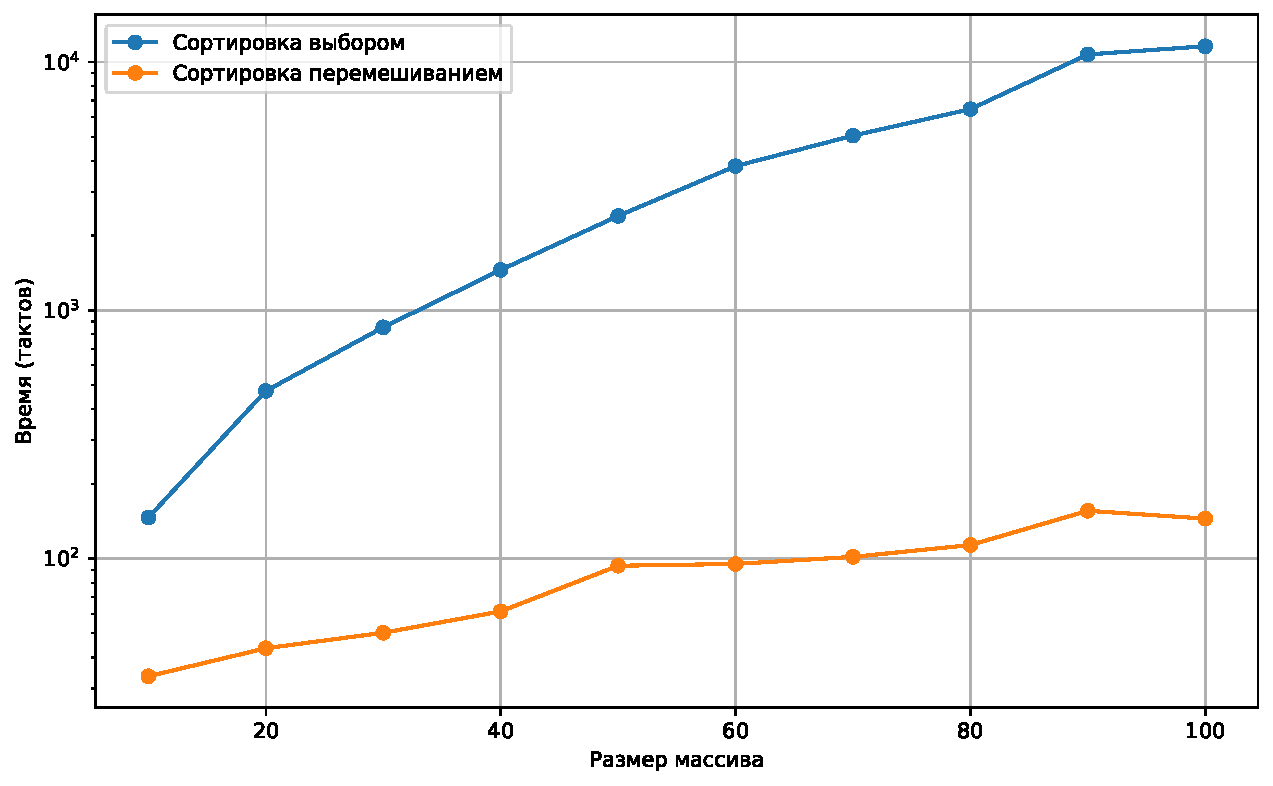
\includegraphics[width=0.9\linewidth]{../src/lab_03/time_logscale}
	\caption{Время выполнения алгоритмов}
	\label{fig:time}
\end{figure}

Сортировка выбором занимает значительно больше времени и уже на 10-ти элементах работает в ~4.35 раза дольше, чем сортировка перемешиванием.
Далее разница увеличивается экспоненциально.

\newpage

\subsection{Занимаемая память реализованных алгоритмов}
 Объём памяти, используемый алгоритмом сортировки целых чисел выбором, равен $4 * N$ байт.
 Алгоритм сортировки перемешиванием занимает на 1 байт больше памяти из-за бинарного флага $swapped$.

\subsection{Вывод}

В результате анализа замеров времени выполнения и затрат памяти на различных алгоритмах были сделаны следующие выводы:

\begin{itemize}
	\item сортировка выбором работает медленнее, чем сортировка перемешиванием;
	\item отношение затраченного времени на сортировку массива увеличивается экспоненциально по мере увеличения размера массива;
	\item сортировка перемешиванием при любом размере массива занимает на 1 байт больше памяти, чем сортировка выбором.
\end{itemize}